\documentclass[journal,twoside]{JoPhA}
\usepackage[utf8]{inputenc}
\usepackage{flushend}
\usepackage{graphicx}


\begin{document}

\title{Predicción de mortalidad en accidentes de tráfico}
 
\author{Samuel Rey y David Moreno
\IEEEcompsocitemizethanks{\IEEEcompsocthanksitem Samuel Rey y David Moreno - Universidad Rey Juan Carlos\protect\\

E-mail: samuel.rey.escudero@gmail.com, dmorenolumb@gmail.com.es
%\IEEEcompsocthanksitem Vicente Matell\'an is with University of Rey Juan Carlos.
} % <-this % s
}


\maketitle


\begin{abstract}
% Yo
	
Resumen
\end{abstract}


%%%%%%%%%% INTRODUCCIÓN %%%%%%%%%%
\section{Introducción}
\IEEEPARstart{L}a predicción de los accidentes de tráfico es uno de los mayores retos de la actual sociedad debido al alto coste económico y, sobre todo, humano que conllevan. Las técnicas de análisis de datos y aprendizaje máquina (\textit{Machine Learning}) ofrecen una oportunidad única para analizar y comprender las razones subyacentes que provocan estos accidentes, otorgando la oportunidad de, en última instancia, predecirlos. En este contexto, los datos recopilados de accidentes anteriores permiten analizar en detalle los factores involucrados para buscar tendencias o patrones. Sin embargo, existen diversos factores que hacen que el análisis de los datos y su utilización para futuras predicciones sea un verdadero reto: \\

\begin{itemize}
	\item Las bases de datos son muy grandes y heterogéneas, por lo que habitualmente no se puede trabajar con datos de distintas procedencias. \\
	
	\item Los datos son introducidos manualmente por personas, por lo que son propensos a errores o valores inádecuado y a presentar ruido. Sobre este tema se profundiza algo más en el artículo \cite{analisis_datos}. \\

	\item Las situaciones reales son complejas y sus datos cuentan con un gran número de atributos, por lo que los modelos utilizados para predecir los resultados tienen una gran dimensionalidad y requieren un gran número de ejemplos. \\
	
	\item Las funciones de coste también suelen ser complejas y altamente no lineales, por lo que es sencillo que el algoritmo e optimización se detenga en un mínimo local. Además, esto ocasiona que el resultado del entrenamiento del modelo dependa en gran medida del punto en el que se inicialicen los pesos al comenzar el entrenamiento. \\
\end{itemize}

% Quitar??
%La utilidad y a la vez, dificultad que esta situación presenta, así como la actual relevancia que está adquiriendo el campo de análisis de datos y aprendizaje máquina, ha motivado la realización de un datatón y concurso en la universidad Rey Juan Carlos. En este datatón se proporcionarán conocimientos básicos en estas materias así como distintos consejos para abordar el problema, haciendo un ranking de las distintas soluciones obtenidas y premiando las dos primeras. \\

En este artículo, para abordar este problema nos centraremos en predecir la gravedad del accidente, abordándolo como un problema de clasificación binaria. Basándonos en los atributos número de heridos leves, número de heridos graves y número de muertos, las clases que hemos definido son: \\

\begin{itemize}
	\item \textit{Clase 0 - Accidente leve}: consideraremos accidetentes leves todos aquellos en los que no haya ni muertos ni heridos.
	\item \textit{Clase 1 - Accidente grave}: clasificaremos como accidentes graves aquellos en los que haya habido muertos o heridos, ya sean leves o graves. \\ 
\end{itemize}



Esta definición de clases ha sido establecida por el concurso organizado en el datatón de la universidad Rey Juan Carlos, y la máquina explicada en este artículo ha sido ha sido propuesta como solución. Esto supone una dificultad añadida, dado que el conjunto de test utilizado para evaluar las diferentes máquinas presentadas al concurso tenía las clases desbalanceadas. Aproximadamente el 75\% de elementos del conjunto de tests pertenecían a la clase 1, mientras que sólo el 25\% representaban a la clase 0. Sin embargo, el conjunto de datos de entrenamiento no estaba desbalanceado. En él, el 54\% de las observaciones pertenecían a la clase 1 y el 46\% restante a la clase 0. \\

La base de datos utilizada consta de más de 9000 observaciones, con 83 atributos cada una. Se trata de datos muy ruidosos y de una gran dimensionalidad, algo que resulta especialmente problemático, como se explica en \cite{alta_dimensionalidad}. Además, la mayoría de los atributos son paramétricos, por lo que presenta pocos outliers. Sin embargo, algunos atributos tenían un gran númro de elementos incorrectos. Todo esto hace que sea necesario una primera fase de procesamiento de datos y selección de características antes de elegir y entrenar el modelo, para utilizar tener en cuenta sólo las características que realmente aportan información y ayudan a mejorar el rendimiento de la máquina. Esta fase de análisis de datos es especialmente importante, dado que evita ayuda a evitar sobreaujustes y que el modelo aprenda errores existentes en los datos o incluso el ruido. Cómo se comenta en \cite{extraccion_datos}, un buen análisis previo puede conseguir que un modelo sencillo supere el rendimiento de modelos mucho más complejos. \\

A continuación, se explicara detalladamente la metodología empleada para resolver el problema. Se explicará en que ha consistido el análisis de datos realizado, los distintos modelos que se han considerado para resolver el problema y las figuras de mérito que hemos considerado. Después, detallaremos los dos modelos que han dado un mejor resultado comentando los parámetros de cada uno, y para finalizar, expondremos las conclusiones a las que hemos llegado después de enfrentarnos a este problema. \\


%%%%%%%%%% METODOLOGÍA %%%%%%%%%%
\section{Metodología}
\IEEEPARstart{P}ara enfrentarnos al problema lo hemos dividido en dos fases distintas. En primer lugar hemos realizado un análisis de datos para solventar datos erróneos y simplificar el problema todo lo posible sin perder información útil. Por otra parte, hemos probado distintos modelos buscando el que mejor se adaptase a los datos consiguiendo mejores resultados. A continuación describiremos estas dos fases en detalle.

\subsection{Análisis de datos}
Al tratarse de datos con una dimensionalidad tan alta y tanto ruido, es imprescindible realizar un buen análisis de los datos y una fase de extracción de características. Para esto, lo primero que hemos hecho ha sido revisar los datos con los que hemos trabajado. De esta forma hemos detectado los atributos que no aportaban información útil para la la clasificación de accidentes, como el \textit{Número de accidente} o el \textit{id}, y los hemos eliminado. Así mismo, hemos detectado atributos en los que más del 90\% de las observaciones tenían un valor de \textit{NaN}, y los hemos elimiado también. Con este primer análisis hemos detectado información repetida. Por ejemplo, los campos \textit{Carretera}, \textit{Km} y \textit{Pk} están ya recogidos en las coordenadas GPS. \\

A continuación, hemos representado cada atributo restante. Al tratarse en su gran mayoría de atributos paramétricos, un gráfico de dispersión no aportaba información. Por lo tanto, hemos utilizado gráficos de barras para visualizar el número de accidentes de cada clase para los distintos valores de los atributos. Con esto, buscábamos encontrar las características que aparentemente no aportasen ningún tipo de información para eleminarlas del conjunto de datos, reduciendo así la dimensionalidad. Sacar estas conclusiones a simple vista no es sencillo y además puede ser erróneo, dado que para algunos atributos podría apreciarse una tendencia al combinarse con otros pero no por separado. Por lo tanto, además de este análisis visual, antes de decidir si borrar o no una característica hemos comparado los resultados obtenidos entrenando la máquina con y sin ella, eliminándola únicamente si no mejoraba el resultado. \\ En la ilustración \ref{fig:graf_tendencia} se muestra un ejemplo de estas gráficas, en la que se observa que la proporción de accidentes en la clase 1 es mayor los sábados y domingos. En contraposición, en la figura \ref{fig:graf_no_tendencia} se muestra un atributo en el que no se observa ninguna tendencia clara.

\begin{figure}[htb!]
	\begin{center}
		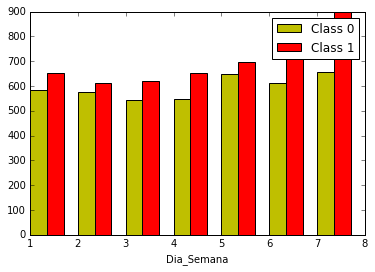
\includegraphics[width=7cm]{figs/dia_semana.png}
		\caption{Número de accidentes en los distintos días de la semana.}
	\end{center}
	\label{fig:graf_tendencia}
\end{figure}
\begin{figure}[htb!]
	\begin{center}
		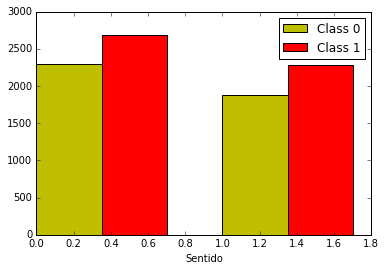
\includegraphics[width=6cm]{figs/hora.png}
		\caption{Número de accidentes dependiendo del sentido doble o no de la vías.}
	\end{center}
	\label{fig:graf_no_tendencia}
\end{figure}

También hemos comprobado la correlación lineal entre los distos atributos utilziando el coeficiente de correlación de Pearson. Si dos atributos tienen una correlación muy alta, significa que existe una dependencia lineal entre ellos, y por lo tanto, comparten la misma información, por lo que podemos prescindir de uno de ellos. En este caso, hemos eliminado los atributos que presentaban una correlción superior al 75\%. De nuevo, hemos comparado los resultados antes y después de eliminar estos atributos para confirmar que no eliminamos nada que perjudique al rendimiento del modelo. \\

Al terminar con este proceso de análisis y extracción de características, hemos reducido los 83 atributos que tenían inicialmente los datos a 61. Aunque ha sido una reducción considerable, la dimensionalidad de los datos aún sigue siendo muy elevada. Por lo tanto, hemos utilizado los siguientes métodos de extracción de características para seleccionar las K mejores: \\

\begin{itemize}
	\item Principal Component Analysis (PCA)
	\item Truncated Singular Value Decomposition (SVD)
	\item Recursive Feature Extraction (RFE)
	\item Información mutua
	\item Mayor varianza \\
\end{itemize}

Para cada método hemos probado diferentes valores de K. Sin embargo, en todos los casos el resultado empeoraba al aplicar la extracción de caraterísticas, consiguiendo mejores figuras de mérito al utilizar todos los valores. \\

\subsection{Selección del modelo}
Después de la extración de características, el principal problema al que nos hemos enfrentado ha sido elegir el modelo más adecuado para este problema de clasificación. Los modelos considerados han sido los sigientes: \\

\begin{itemize}
	\item MLP
	\item SVM
	\item K-vecinos
	\item PNN
	\item Regresor logístico \\
\end{itemize} 

Sabiendo que el conjunto de test está desbalanceado, hemos considerado que la exactitud o \textit{accuracy} no era la mejor métrica para evaluar el rendimiento de los modelos, y hemos decidido utilizar la precisión o \textit{precision}. Inicialmente dividimos los datos en 10 grupos y usamos la función \textit{cross\_val\_score} proporcionada por la librería \emph{sk-learn}\cite{validacion_cruzada}, fijándonos en la media y la desviación estándar para comparar los resultados de los distintos modelos. Sin embargo, consideramos que el número de observaciones era suficientemente grande, por lo que finalmente empleamos la división simple para su valuación. De esta forma, además de agilizar el proeceso de evaluación, la información que conseguíamos de cada realización era más detallada. Utilizamos la función \textit{classification\_report}, que basándose en la información de la matriz de confusión ofrece información sobre la precisión, sobre el \textit{recall} y el \textit{F1 score}, de cada clase y en media. \\

Para la evaluación de los modelos, el 80\% de los datos disponibles se han utilizado para entrenar el modelo (conjunto de entrenamiento) y el 20\% restante para evaluarlo (conjunto de validación). La separación de estos grupos se ha realizado de forma aleatoria y se ha supuesto que únicamente conocíamos los datos de entrenamiento, tratando el conjunto de validación como el conjunto de test. \\

Después de definir estos conjuntos y el método empleado para la evaluación, empezamos a probar los distintos modelos anteriormente mencionados. Cada uno de estos modelos cuenta con unos parámetros distintos que hay que ajustar para que las prediciones de la máquina sean lo más precisas posibles. Para esto, seleccionamos los valores para los parámetros que consideramos más adecuados, entrenamos la máquina con el conjuto de entrenamiento y evaluamos su rendimiento utilizando el conjunto de validación. Con esta información, reajustamos los valores buscando siempre minimizar el error en el conjunto de validación, no en el de entrenamiento. Además, al haber más muestras de la clase 1 que de la clase 0 en el conjunto de validación, nos centramos sobre todo en conseguir una precisión elevada en la clase 1. De esta forma asumimos costes asimétricos, dado que asignar a una observación la clase 0 cuando en realidad pertenecía a la clase 1 tenía un coste muy alto, mientras que, un falso positivo de la clase 1 no tenía tanto coste. \\

Finalmente, cuando estuvimos satisfechos con la precisión obtenida con una determinada determinada configuración del modelo, utilizamos el 100\% de los datos para entrenar la máquina, obtenemos las predicciones del conjunto de test y comprobamos los resultados. Teóricamente, con esto añadimos más datos al modelo al estar utilizando todas las observaciones disponibles, por lo que conseguiremos que generalice mejor y se sobreajuste menos a los datos con los que se ha entrenado, obteniendo por lo tanto resultados ligeramente mejores. \\


%%%%%%%%%% RESULTADOS %%%%%%%%%%
\section{Resultados}
\IEEEPARstart{E}n este capítulo hemos seleccionado los dos modelos que han dado mejores resultados, de todos los mencionados en el capítulo anterior. Para cada uno de ellos explicaremos la configuración de sus parámetros, las técnicas que hemos utilizado en su aprendizaje y expondremos los resultados que hemos obtenido con ellos.


\subsection{SVM}
	% David

\subsection{MLP}
	% Yo


\section{Conclusiones}
% David

\begin{thebibliography}{1}

\bibitem{analisis_datos}
Figuera, C., Lillo, J. M., Mora-Jimenez, I., Rojo-Álvarez, J. L., \& Caamaño, A. J. (2011, October). \emph{Multivariate spatial clustering of traffic accidents for local profiling of risk factors.} In Intelligent Transportation Systems (ITSC), 2011 14th International IEEE Conference on (pp. 740-745). IEEE.

\bibitem{extraccion_datos}
Mitchell, T. M. (2006). \emph{The discipline of machine learning (Vol. 9).} Carnegie Mellon University, School of Computer Science, Machine Learning Department.

\bibitem{alta_dimensionalidad}
Domingos, P. (2012). \emph{A few useful things to know about machine learning.} Communications of the ACM, 55(10), 78-87.

\bibitem{validacion_cruzada}
\emph{Cross-validation: evaluating estimator performance} http://scikit-learn.org/stable/modules/cross\_validation.html

\end{thebibliography}
\end{document}


